\documentclass{standalone}
\usepackage{tikz}
\usepackage{ctex,siunitx}
\usepackage{tkz-euclide}
\usepackage{amsmath}
\usetikzlibrary{patterns, calc}
\usetikzlibrary {decorations.pathmorphing, decorations.pathreplacing, decorations.shapes,}
\begin{document}
\small
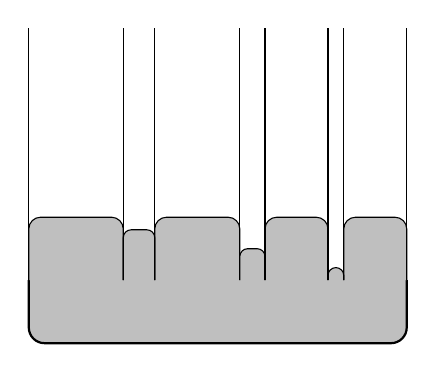
\begin{tikzpicture}[>=stealth,scale=0.8]
  \draw [fill=gray!50, rounded corners=0.2cm, thick](0,1)--(0, 0)--(6,0)--(6,1);
  \draw [fill=gray!50, rounded corners=0.15cm](0,1)--(0,2)--(1.5,2)--(1.5,1);
  \draw [fill=gray!50, rounded corners=0.15cm](2,1)--(2,2)--(3.35,2)--(3.35,1);
  \draw [fill=gray!50, rounded corners=0.15cm](3.75,1)--(3.75,2)--(4.75,2)--(4.75,1);
  \draw [fill=gray!50, rounded corners=0.15cm](5,1)--(5,2)--(6,2)--(6,1);
  \draw [fill=gray!50, rounded corners=0.1cm](1.5, 1)--(1.5,1.8)--(2, 1.8)--(2,1);
  \draw [fill=gray!50, rounded corners=0.1cm](3.35, 1)--(3.35,1.5)--(3.75, 1.5)-- (3.75, 1);
  \draw [fill=gray!50, rounded corners=0.1cm](4.75, 1)--(4.75, 1.2)--(5, 1.2)--(5, 1);
  \foreach \x in {0,1.5,2,3.35,3.75,4.75,5,6}
  {
    \draw (\x, 1)--(\x, 5);
  }
\end{tikzpicture}
\end{document}